% -----------------------------------------------------------------
% 2. WBS Dictionary
% -----------------------------------------------------------------
\section{WBS Dictionary}

\subsection{Datos Generales}

\begin{tabularx}{\textwidth}{@{}lX@{}}
\textbf{Project Title:} & Hub Financiero \\
\textbf{Date Prepared:} & 21/08/2025 \\
\textbf{Work Package Name:} & 1.5.1 Mobiliario \\
\textbf{Code of Accounts:} & 1.5.1 \\
\end{tabularx}

\subsection{Relación con el EDT}

La información de este diccionario corresponde al paquete de trabajo \textbf{1.5.1 Mobiliario} del EDT del proyecto (véase la Figura~\ref{fig:edt}).

\begin{figure}[H]
  \centering
  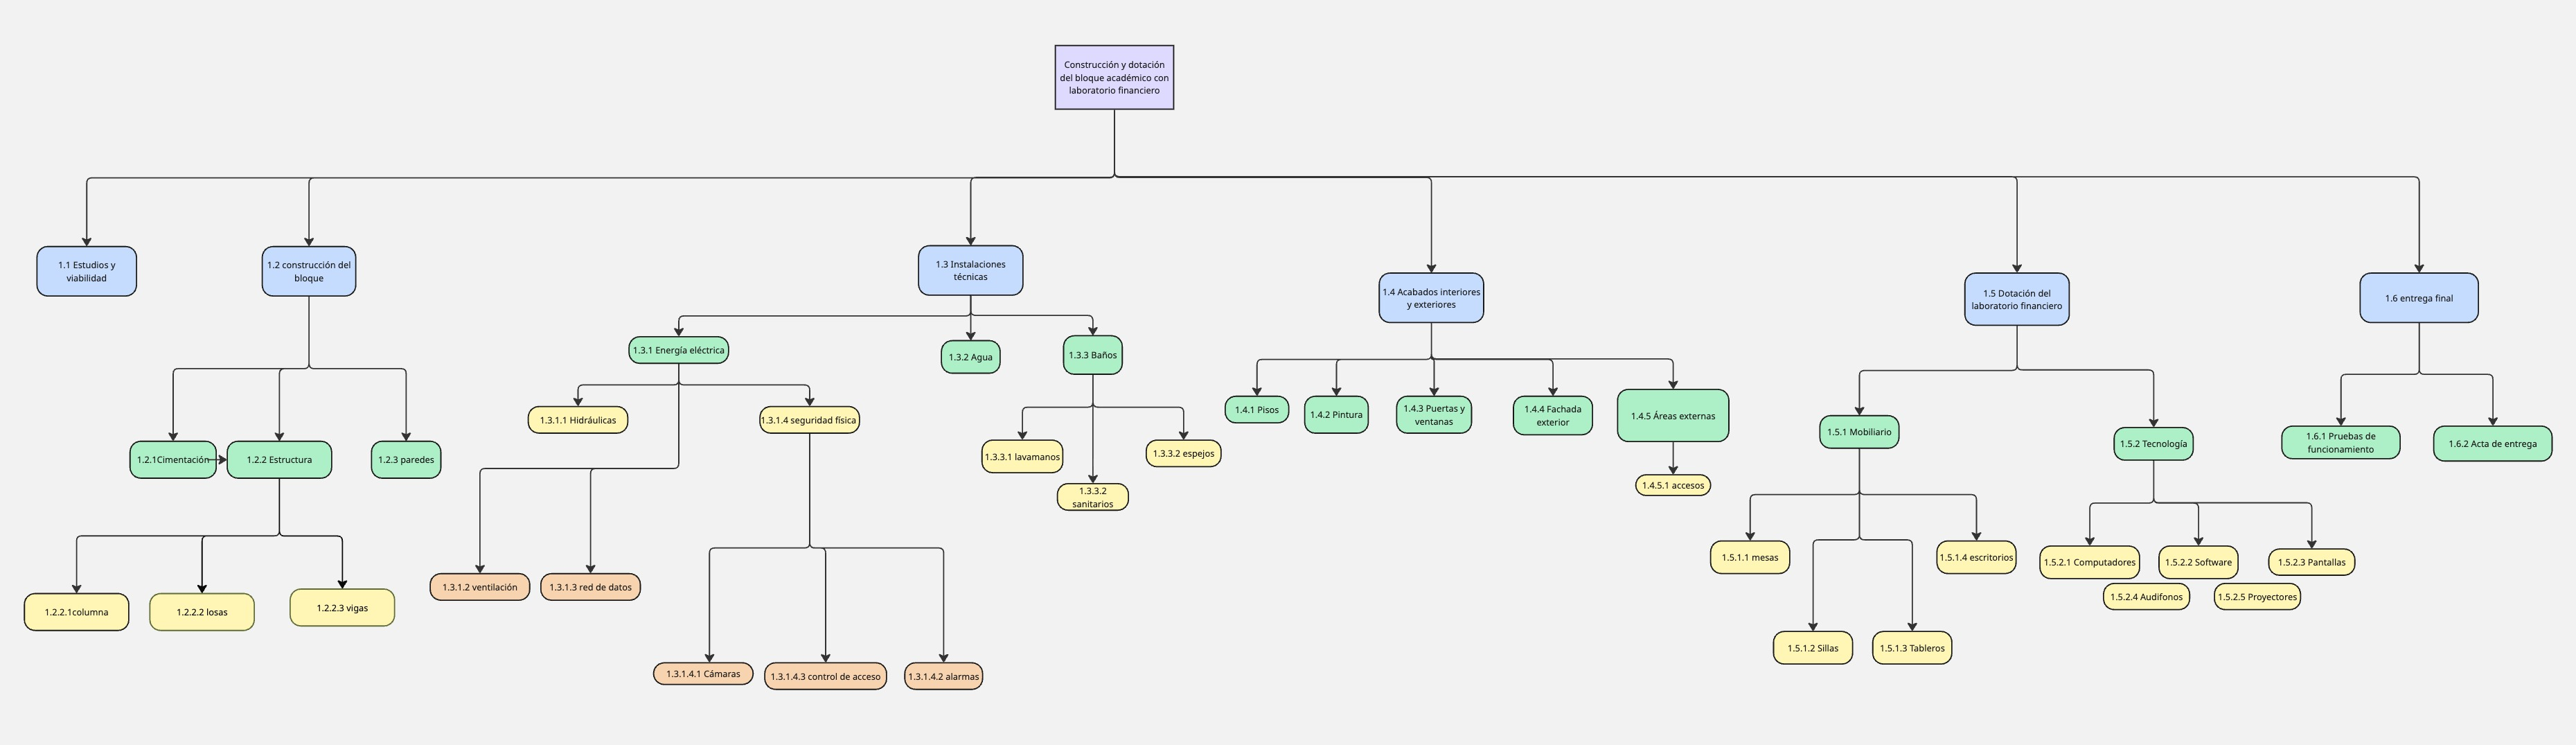
\includegraphics[width=\textwidth]{Figures/0. General/EDT.jpg}
  \caption{Estructura de Desglose del Trabajo (EDT) del proyecto.}
  \label{fig:edt}
\end{figure}

\subsection{Descripción del Paquete de Trabajo}

Este paquete corresponde a la dotación de mobiliario del laboratorio financiero, incluyendo mesas, sillas, tableros y escritorios. Su propósito es garantizar espacios adecuados, ergonómicos y estéticos para el aprendizaje y la práctica académica de los estudiantes.

\subsection{Supuestos y Restricciones}

\begin{itemize}
    \item Se asume que los proveedores entregarán dentro de los plazos establecidos.
    \item Se asume que los precios se mantendrán dentro de los rangos pactados.
    \item La instalación debe realizarse en el sitio final de uso con supervisión de la Universidad.
    \item Restricción: el mobiliario debe cumplir estándares de ergonomía y resistencia aprobados por la Universidad.
\end{itemize}

\subsection{Actividades y Detalles}

% Nota: usamos p{<ancho>} con \parbox en el encabezado para evitar cortes de texto.
\begin{longtable}{|>{\raggedright\arraybackslash}p{1.2cm}|
                        >{\raggedright\arraybackslash}p{1.8cm}|
                        >{\raggedright\arraybackslash}p{2.2cm}|
                        >{\raggedright\arraybackslash}p{2.8cm}|
                        >{\raggedright\arraybackslash}p{2.2cm}|
                        >{\raggedright\arraybackslash}p{4.4cm}|}
\hline
\textbf{WBS ID} &
\textbf{Elemento} &
\textbf{Proveedor} &
\textbf{Costo Unitario (COP)} &
\textbf{Fecha Entrega} &
\textbf{Criterio de Aceptación} \\
\hline
\endfirsthead
\hline
\textbf{WBS ID} &
\textbf{Elemento} &
\textbf{Proveedor} &
\textbf{Costo Unitario (COP)} &
\textbf{Fecha Entrega} &
\textbf{Criterio de Aceptación} \\
\hline
\endhead
1.5.1.1 & Mesas & Mesas y Sillas Medellín SAS &
900,000 -- 1,600,000 & 10 Nov 2026 &
Mesas blancas hechas a la medida, con instalación por el productor. Entrega el mismo día pactado. \\
\hline
1.5.1.2 & Sillas & Mesas y Sillas Medellín SAS &
250,000 -- 400,000 & 12 Nov 2026 &
Sillas ergonómicas color negro que brinden comodidad y estética. Instalación completa en salones. \\
\hline
1.5.1.3 & Tableros & Todo Acrílico SAS &
300,000 -- 800,000 & 13 Nov 2026 &
Tableros acrílicos limpios e instalados en pared o soporte, listos para presentaciones y simulaciones. \\
\hline
1.5.1.4 & Escritorios & Scribtorios SAS &
250,000 -- 500,000 & 15 Nov 2026 &
Escritorios individuales con silla incorporada, de plástico resistente. Precio negociado en 250,000 por contrato e instalación completa en aulas. \\
\hline
\end{longtable}

\subsection{Requisitos de Calidad}

\begin{itemize}
    \item Todo el mobiliario debe cumplir normas de seguridad y ergonomía.
    \item Materiales resistentes al uso intensivo y de fácil mantenimiento.
    \item Garantía mínima de 2 años por defectos de fábrica o instalación.
\end{itemize}

\subsection{Criterios de Aceptación}

El paquete de mobiliario será aceptado si:
\begin{itemize}
    \item Todos los elementos son entregados en la fecha establecida.
    \item La instalación es completa y funcional en las aulas asignadas.
    \item Se cumplen los estándares de ergonomía, seguridad y estética.
\end{itemize}

\subsection{Información Técnica}

\begin{itemize}
    \item Mesas y escritorios de superficie plástica resistente, fáciles de limpiar.
    \item Tableros acrílicos con instalación fija a muro o soporte.
    \item Sillas ergonómicas de color negro, acolchadas, con soporte metálico.
\end{itemize}

\subsection{Información de Acuerdos}

\begin{itemize}
    \item Los contratos con proveedores incluyen instalación y transporte.
    \item El precio de escritorios fue previamente negociado a 250,000 COP.
    \item Los proveedores deben emitir certificados de garantía y cumplimiento.
\end{itemize}
